% `template.tex', a bare-bones example employing the AIAA class.
%
% For a more advanced example that makes use of several third-party
% LaTeX packages, see `advanced_example.tex', but please read the
% Known Problems section of the users manual first.
%
% Typical processing for PostScript (PS) output:
%
%  latex template
%  latex template   (repeat as needed to resolve references)
%
%  xdvi template    (onscreen draft display)
%  dvips template   (postscript)
%  gv template.ps   (onscreen display)
%  lpr template.ps  (hardcopy)
%
% With the above, only Encapsulated PostScript (EPS) images can be used.
%
% Typical processing for Portable Document Format (PDF) output:
%
%  pdflatex template
%  pdflatex template      (repeat as needed to resolve references)
%
%  acroread template.pdf  (onscreen display)
%
% If you have EPS figures, you will need to use the epstopdf script
% to convert them to PDF because PDF is a limmited subset of EPS.
% pdflatex accepts a variety of other image formats such as JPG, TIF,
% PNG, and so forth -- check the documentation for your version.
%
% If you do *not* specify suffixes when using the graphicx package's
% \includegraphics command, latex and pdflatex will automatically select
% the appropriate figure format from those available.  This allows you
% to produce PS and PDF output from the same LaTeX source file.
%
% To generate a large format (e.g., 11"x17") PostScript copy for editing
% purposes, use
%
%  dvips -x 1467 -O -0.65in,0.85in -t tabloid template
%
% For further details and support, read the Users Manual, aiaa.pdf.


% Try to reduce the number of latex support calls from people who
% don't read the included documentation.
%
\typeout{}\typeout{If latex fails to find aiaa-tc, read the README file!}
%

\documentclass[]{aiaa-tc}% insert '[draft]' option to show overfull boxes

\usepackage{graphicx}
\usepackage{float}

 \title{Iterative Time Reversal in Dispersive and Non-Dispersive Mediums}

 \author{
  Brian C. Fehrman
    \thanks{Advanced Dynamics Laboratory, Research Assistant, Mechanical Engineering Department, 501 E. St. Joseph Street, Rapid
City, SD 57701, AIAA Student Member.}
  \ and Alexander J. Cushman \thanksibid{1}\\
  \ and Umesh A. Korde%
   \thanks{Professor, Mechanical Engineering Department, 501 E. St. Joseph Street, Rapid City, SD 57701, AIAA Member.}\\
 }

 % Data used by 'handcarry' option if invoked
 \AIAApapernumber{YEAR-NUMBER}
 \AIAAconference{Conference Name, Date, and Location}
 \AIAAcopyright{\AIAAcopyrightD{YEAR}}

 % Define commands to assure consistent treatment throughout document
 \newcommand{\eqnref}[1]{(\ref{#1})}
 \newcommand{\class}[1]{\texttt{#1}}
 \newcommand{\package}[1]{\texttt{#1}}
 \newcommand{\file}[1]{\texttt{#1}}
 \newcommand{\BibTeX}{\textsc{Bib}\TeX}

\begin{document}

\maketitle

\begin{abstract}
In this paper we further investigate acoustic energy as a tool to enhance the recovery rate of a self healing material. Time reversal is the method used for the focusing of acoustic energy at a recovering location. Our recent tests, which have produced promising results, included applying acoustic time reversal in an iterative fashion in order to focus and amplify a stress-wave at a defect within a solid rod. Two types of rods were used for testing; (i) a solid steel rod (non-dispersive) and (ii) a brass tube filled with a fully cured two-part epoxy (dispersive). The curing of a two-part epoxy is treated as being analogous to the curing of a self healing material. We have continued to look at the effects of acoustic energy on the curing of the epoxy. It was found that the curing rate of the epoxy was accelerated with the introduction of acoustic energy.
\end{abstract}


\section{Introduction}

Many times it is taken for granted that machines and structures will be accessible for repair in the event that damage occurs. When it comes to space structures, however, we are not afforded the convenience of reasonably easy access in order to repair damages. Damage to space structures can occur quite frequently in the form of surface cracks as a result of collisions with mirco-meteroids or space debris. Materials with the ability to heal themselves are very desirable for this application \cite{Lee2009}. 

There has been a large interest in self healing materials recently. Some of this work applies biological concepts to the problem \cite{Blaysik2010}. The rate of recovery is of importance because the damage in the material may be able to continue its growth while the material is attempting to mend itself. If the damage expands quicker than the material is able to heal itself, then the material may never reach full mechanical recovery.  A lot of the research performed on accelerating the recovery rate has looked at the problem from a materials level \cite{White2001, Sheng2009, Burattini2009, Nakao2009, Fettig2009, Imperiale2009, Zhang2007}. Heating the material, cooling the material, and introducing ultra-violet light are other methods that have been used to speed the healing of the material \cite{Sloof2009, Song2009, Bosman2009, Djugum2009, Murphy2009, Garcia2009}. Calculations based on work by Wool and O'Connor have shown that increasing the pressure at a recovery site will increase the rate of that recovery \cite{Wool1981, Barnes2009, Sarrazin2009}. It is our goal to use acoustic energy to increase the localized pressure at a damaged location in order to speed its recovery rate. 

In the interest of efficiency, we aim to focus the energy at the recovery site rather than arbitrarily sending it throughout the whole material. In addition to power considerations, focusing the energy is important because a large amount of unfocused energy could damage the structure even further. Time reversal is the method we choose to focus acoustic energy at a recovering location. One of the many advantages of this method is that no actual knowledge of the damaged location is ever needed for the algorithm to work. Time reversal is not a new concept and many implementations of it have been studied \cite{ Anderson2008, Borcea2003, Fink2009, Sutin2004, Harley2009}.  One implementation of time reversal allows for it to be applied iteratively. Better focusing is achieved with each iteration of the time reversal. 

In this paper we continue our studies on time reversal in solid rods \cite{AIAASelfHeal2011}. This time, however, we apply iterative time reversal to both a non-dispersive and a dispersive rod. Each rod has a defect location in which we wish to focus acoustic energy. Due to the difference between the rod mediums, a slightly different form of iterative time reversal is applied to each rod. These experiments bring us another step closer to directly testing the effects of using time reversal to focus energy at a recovering location. We have also performed further tests on the two-part epoxy curing without and with unfocused acoustic energy being introduced into the system.

\section{Experimental Implications}

For us to further our work on accelerating the healing rate of a damaged location, we continue to look at what we feel are the two most important aspects of the project; (i) how the recovery rate of a self healing material is affected by the introduction of acoustic energy and (ii) how to best focus the acoustic energy at a recovering site. We take care of the first item by our continued studies on epoxy curing. As shown by Wool and O'Connor, epoxy curing is analogous to self healing recovery because of the fact that they both go through the same five stages when recovering which are: (a) surface rearrangement, (b) surface approach, (c) wetting, (d) diffusion, and (e) randomization. New experimental setups using time reversal have helped to further address the second item of how to focus the acoustic energy.

\subsection{Epoxy Curing Experiments}
The setup and experiments used for the epoxy curing experiments have largely remained the same. We fill brass tubes with a two-part epoxy and then monitor the curing process of the epoxy. There are two objective ways that the state of epoxy is characterized; (i) the temperature of the epoxy and (ii) the vibrational response of the epoxy. A thermistor embedded within the epoxy before the curing begins provides a temperature reading of the epoxy throughout the curing process. A marble dropper is used to cause a vibrational response in the epoxy-filled brass tube and is recorded using an accelerometer attached to the outside of the tube. New software has been written for the data acquisition which provides for more reliable testing and easier data manipulation. This new software, which is written in LabVIEW, also uses different hardware than what was used previously. This has enabled us to have better control over acquiring the different measurements needed for our experiments. This entire setup is still housed within a wooden box which allows us to control the ambient temperature of the experiment which provides us with more consistent results. 

Our experiments look at the rate at which the epoxy cures without and with acoustic excitation. A speaker placed on top of the box mentioned above introduces the acoustic excitation into the system. These setups, minus the box and marble dropper, are shown in Figures \ref{fig:epoxy_no_sound} and \ref{fig:epoxy_sound}

\begin{figure}[H]% order of placement preference: here, top, bottom
\centering
 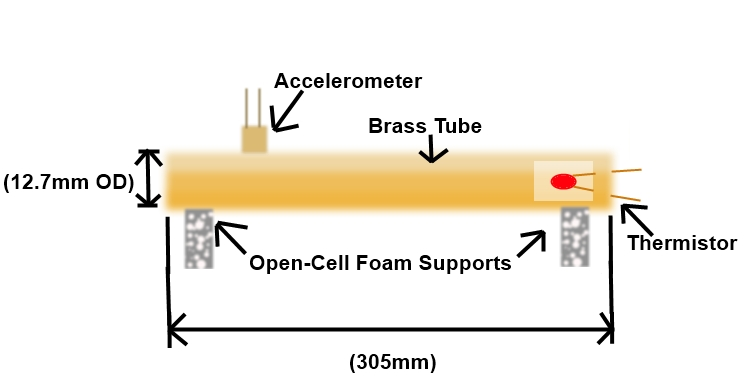
\includegraphics{epoxy_diagram_new}
 \caption{Diagram showing the setup and dimensions of the epoxy curing experiment without acoustic excitation}
 \label{fig:epoxy_no_sound}
\end{figure}


\begin{figure}[H]% order of placement preference: here, top, bottom
\centering
 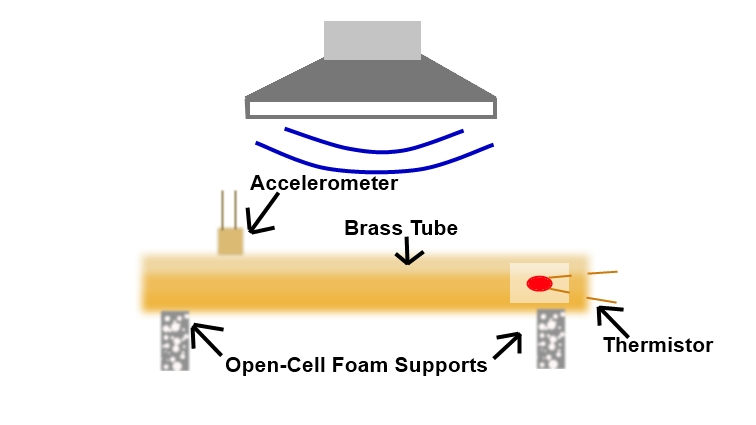
\includegraphics[height = 8cm]{epoxy_diagram_new_speaker}
 \caption{Diagram showing the setup of the epoxy curing experiment with acoustic excitation. Please note that the dimensions of the rod setup are the same as those shown in the previous figure. Speaker not to scale.}
 \label{fig:epoxy_sound}
\end{figure}


\subsection{Iterative Time Reversal Experiments}

In these experiments we continue to use solid, circular rod segments which simplify both analysis and experimental design. The ceramic piezoelectric transducers (PZTS) are still used to send and receive ultrasonic signals. One PZT acts as the defect location and is placed between the ends of the two rod segments (Defect PZT). PZTs are then placed on each open end of the rod segments (Ch0  PZT and Ch1 PZT) for a total of three PZTs used. This system is then placed under compression. The dimensions of the experimental setup are shown in Figure \ref{fig:tr_dimensions}.

\begin{figure}[H]% order of placement preference: here, top, bottom
\centering
 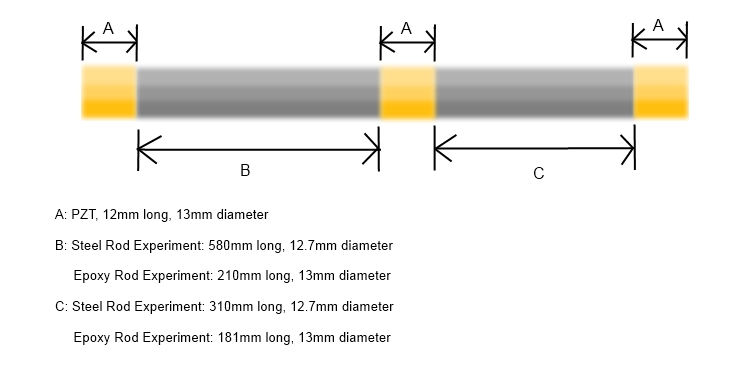
\includegraphics[height = 9cm]{tr_dimensions_new}
 \caption{Diagram showing the setup and dimensions of the time reversal experiment}
 \label{fig:tr_dimensions}
\end{figure}

Instead of just solid steel rods, however, we now introduce time reversal tests using the same epoxy filled brass tubes that are used in the epoxy curing experiments. This material provides much more dispersion than does the steel. For this reason, we consider the solid steel rods to be non-dispersive and the epoxy filled brass tubes to be dispersive. It should be noted that the epoxy in the brass tubes is in its fully cured and hardened state for these experiments. 

The time reversal algorithm used in these experiments has also changed. In the algorithm used before, a signal is sent out from the Ch0 PZT. This signal propagates through the first rod segment and towards the Defect PZT. When the signal reaches the Defect PZT, part of its energy is reflected back towards Ch0 PZT and part of it continues its propagation through the other rod segment and towards the Ch1 PZT. These reflected and transmitted signals are recorded by the Ch0 PZT and the Ch1 PZT, respectively. These recorded signals are then amplified and played back in a time reversed fashion such that they meet and combine at the point where they originally split apart (i.e., the Defect PZT). This implies a focusing of their energy at that location. This is where our previous experiments would end. In the newest experiments we apply this process iteratively which causes the focusing to increase with each iteration. Due to the difference between the dispersive and non-dispersive materials, the algorithm used for each one is slightly different. The flowchart for both time reversal algorithms is shown in Figure \ref{fig:tr_flowchart}.

\begin{figure}[H]% order of placement preference: here, top, bottom
 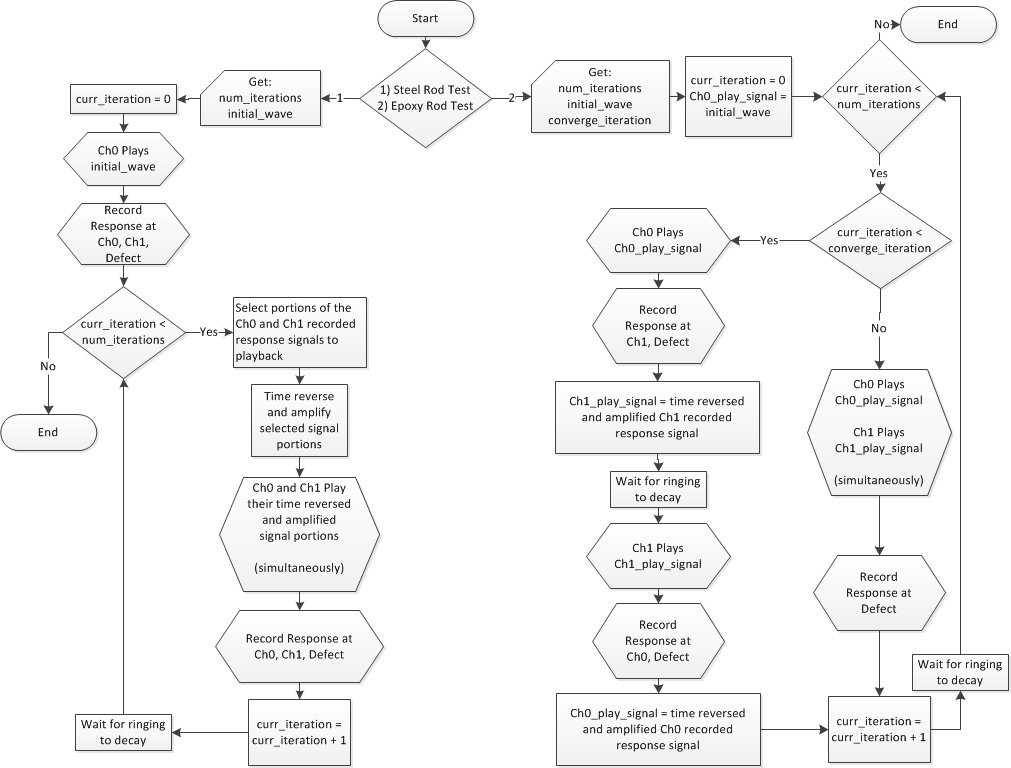
\includegraphics{tr_flowchart}
 \centering
 \caption{Diagram showing the setup and dimensions of the time reversal experiment}
 \label{fig:tr_flowchart}
\end{figure}


\section{Experimental Results}
Our self healing experiment studies consist of two main parts; (i) epoxy curing and (ii) time reversal. In order to achieve our goal of accelerating the recovery rate of a self healing material, we need to first show that acoustic excitation increases the curing rate of the epoxy and also show that time reversal increases acoustic energy focusing at a defect location. 

\subsection{Epoxy Curing Results}

As mentioned previously, one of the measures used to characterize the state of the curing epoxy within the brass tube is its vibrational response to a marble being dropped on it. This response is recorded via an accelerometer placed on the outside of the tube. The FFT of this response is then plotted. As the epoxy cures, the frequencies that it responds greatest to will shift. This can be seen on the FFT graph as the peaks moving from one frequency to another and/or growing in amplitude. Thus, by looking at the peaks on the FFT plot we can see how close the material is to being cured at any given point. This provides a good way to compare the rate of curing for the epoxy without and with acoustic excitation. Figure \ref{fig:epoxy_fft_no_sound} shows the FFT of the vibrational response of the epoxy without acoustic excitation at 2 hours and the FFT at its fully cured state. Figure \ref{fig:epoxy_fft_sound} shows the same FFTs except acoustic energy has been introduced into the system in order to excite the epoxy during the cure process. We can see that when the acoustic energy is used, the epoxy is much closer to its final cured state after 2 hours than it is without using the acoustic energy. This leads us to believe that the acoustic energy does increase the rate of the epoxy curing.

\begin{figure}[H]% order of placement preference: here, top, bottom
\centering
 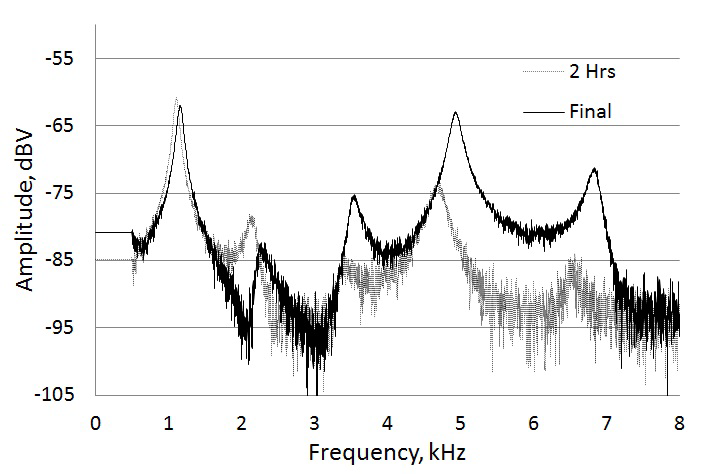
\includegraphics[height = 8cm]{epoxy_fft_no_sound}
 \caption{FFT of the vibrational response of the epoxy filled brass tube 2 hours into cure and in its final state without using acoustic energy}
 \label{fig:epoxy_fft_no_sound}
\end{figure}

\begin{figure}[H]% order of placement preference: here, top, bottom
\centering
 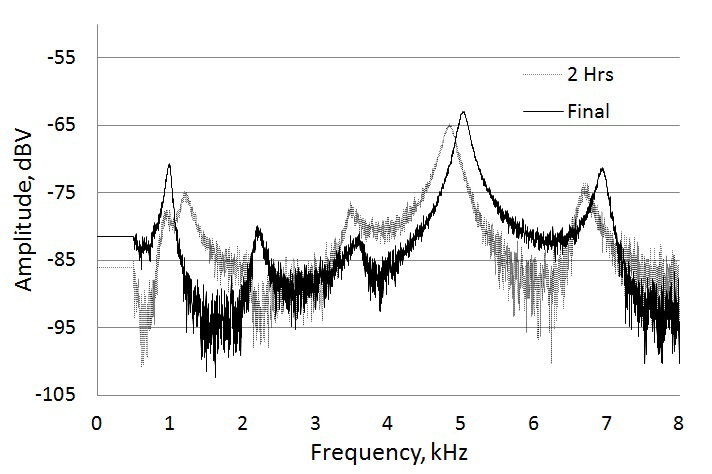
\includegraphics[height = 8cm]{epoxy_fft_sound}
 \caption{FFT of the vibrational response of the epoxy filled brass tube 2 hours into cure and in its final state with acoustic energy introduced}
 \label{fig:epoxy_fft_sound}
\end{figure}

\subsection{Time Reversal Results}

In both the steel rod and epoxy rod experiments we saw an increase in the amplitude of the response recorded at the Defect PZT by using the iterative time reversal. With the steel rod experiments we saw a very close match between the analytical and experimental results.  

Figure \ref{fig:tr_steel2} shows the results of time reversal being applied iteratively. You can see that the signal has been significantly increased by the 6th iteration. 

\begin{figure}[H]% order of placement preference: here, top, bottom
\centering
 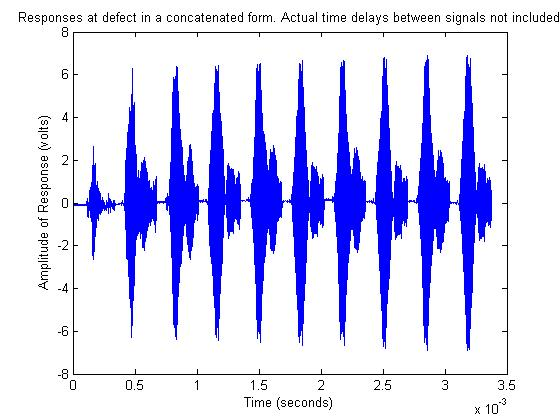
\includegraphics[height = 8cm]{tr_steel_rod_results}
 \caption{Graph of the experimental results of the response at the defect through successive iterations of the time reversal algorithm. You can see that the wave grows larger with each iteration. The secondary wave is thought to result from the adhesive used to couple the rod and PZTs.}
 \label{fig:tr_steel2}
\end{figure}

Even with the dispersion effects of the epoxy, results similar to that of the steel rods can be seen in these experiments. It is seen that the amplitude of the defect response grows with each iteration. Figure \ref{fig:tr_epoxy1} shows the graph of the response at the defect for each iteration.

\begin{figure}[H]% order of placement preference: here, top, bottom
\centering
 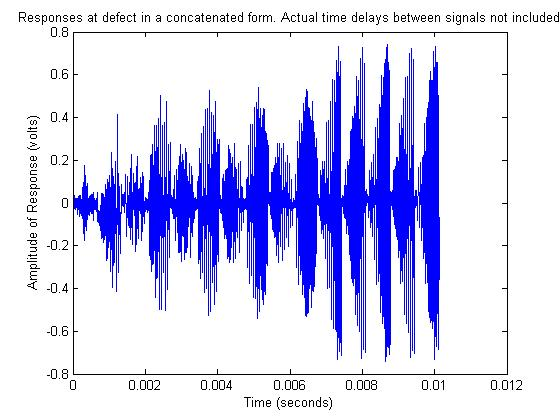
\includegraphics[height = 8cm]{tr_epoxy_results}
 \caption{Graph showing the results of the iterative time reversal used with the epoxy filled brass tubes. You can see that the wave grows larger and larger after each iteration.}
 \label{fig:tr_epoxy1}
\end{figure}


\section{Conclusion and Future Work}

In our epoxy experiments we have seen that the rate of curing is increased with the introduction of acoustic energy. The time reversal experiments strongly suggest that we can achieve a focusing and thus an increase in pressure at a defect location. By applying time reversal in an iterative fashion we are able to further increase the amplitude of that response. We have been able to achieve the same results in a dispersive medium where as before we were testing solely with a non-dispersive medium. Further tests will include testing the time reversal in multiple dimensions. We will also combine the epoxy curing and time reversal experiments in an attempt to increase the curing rate by focusing acoustic energy.

\section{Acknowledgments}

We would like to thank the ARL for their support. Also, we would like to thank Dr. Chris Jenkins from Montana State University for his input. Thanks are also due to Dr. Jeffry Welsh and Mr. Jeremy Banik from the AFRL for their suggestions.

\bibliography{references}{}
\bibliographystyle{unsrt}

\end{document}
